\documentclass[11pt]{scrartcl}

\usepackage{ucs}
\usepackage[utf8x]{inputenc}
\usepackage{ngerman}
\usepackage{amsmath,amssymb,amstext}
\usepackage{graphicx}
\usepackage[automark]{scrpage2}
\usepackage{pgfplots}
\usepackage{chngcntr}
\usepackage[left=3cm, right=3cm, top=3cm, bottom=3cm]{geometry}
\counterwithin{figure}{section}

\pagestyle{scrheadings}

\title{Binärer Suchbaum}
\author{Finn Jannsen, Philipp Schwarz}
\date{\today{}}

\begin{document}

\maketitle

\tableofcontents

\section{Einführung}
	\label{sec:einfuehrung}
	
	Diese Dokumentation beschreibt Implementationen für binäre Suchbäume.
	In Abschnitt \ref{sec:implementation} wird darauf eingegangen, wie der Algorithmus realisiert wurde.
	Anschließend wird in Abschnitt \ref{sec:veri} geprüft, ob die Implementation korrekt funktioniert 
	und in Abschnitt \ref{sec:aufwand} die Performance mit dem zu Grunde liegenden Quicksort verglichen.

\section{Implementation}
	\label{sec:implementation}
	
	Der Algorithmus wurde als Klasse realisiert, der ein Interface implementiert, welches es ermöglicht, einfach weitere Implementationen, sofern dies gewünscht wird, zu schreiben.
	
	\subsection{Aufbau}
		\label{sec:codeStruc}
		
		Die zu Grunde liegende Aufgabe bestand aus 2 Teilen. Im ersten ging es darum, einen binären Suchbaum zu implementieren, welcher Als Elemente Generics entgegen nimmt.
		Unter anderem sollte der Baum einmal aus verlinkten Nodes (dt. Knoten) bestehen und einmal in einen Array eingebettet sein. Letzteres unterstützt nur geringe Baumgrößen, da die Indexe von Childs (dt. Kinder) $2*i$ aufwärts sind, wobei $i$ der Index von dem Father-Node ist. 
		Das sorgt relativ schnell für interne Integer-Overflows, wobei das Java-Framework auch nur Integer-Größen als Array-Größen akzeptiert.
		Diese Implementation wurde erfolgreich durchgeführt mit Generics, die "Comparable" implementieren, denn um den Baum sortiert zu erstellen müssen die Elemente miteinander verglichen werden.
		Der Baum sollte im zweiten Teil so umgebaut werden, dass er Integer als Elemente akzeptiert. Außerdem sollte folgende Funktionalität hinzugefügt werden:\\\\
		\textbf{Eingabe}: Zwei natürliche Zahlen $m$ und $M$\\
		\textbf{Ausgabe}: $\sum_{i}a_i$ $m \leq a_i \leq M$\\

		Da die Array-Einbettung erhebliche Performance-Nachteile hat, was den effizienten Speichergebrauch angeht, wird im nachfolgenden das Augenmerk auf die verkettete Node-Implementation gelegt.
		Die Nodes haben jeweils 3 Verweise auf Nodes: Father-, Left- und Right-Node. Die letzten beiden sind die Childs. 
		Um die gefordete Funktionalität zu erfüllen wurden im zweiten Aufgabenteil außerdem 2 zusätzliche Integer beigefügt: \\
		\textbf{bSum}, die Summe des Branch (dt. Zweig) inkl. aller Child-Nodes und \textbf{sum}, die Summe aller kleineren Elemente einschließlich des Nodes selbst.
		\textbf{bSum} wird beim hinzufügen eines Nodes geupdatet. Dafür ruft der hinzugefügte Node eine Methode auf, die rekursiv über die Father-Nodes bishin zum Root-Node die Werte aktualisiert. Der Code ist unter \ref{figure:bSum} zu sehen.
		\textbf{sum} wird nach dem Hinzufügen einer oder mehrerer Nodes geupdated. Die dazugehörige Methode läuft rekursiv vom Root-Node über alle Child-Nodes und aktualisiert \textbf{sum}. Dabei wird wie in \ref{figure:sum} zu sehen \textbf{bSum} zur Hilfe genommen.

	\subsection{Algorithmus}
		\label{sec:algo}

		Der eigentliche Algorithmus zum Berechnen der Summe aller Nodes zwischen $m$ und $M$ ist durch die in \ref{sec:codeStruc} erklärten Zusatzinformationen sehr simpel.
		Im Grunde genommen besteht das Ergebnis aus den Werten von den 2 nächsten Nodes zu $m$ und $M$ und berechnet sich wie folgt:
		\begin{equation*}
		\sum_{i}a_i = right.sum - (left.sum - left.key)
		\end{equation*}
		Der dazugehörige Code ist unter \ref{figure:sumCalc} zu sehen. Hier wird auch eine weitere Methode ersichtlich, die zum finden der richtigen Knoten für die Berechnung anhand $m$ und $M$ benötigt wird.
		Sie sucht vom Root-Node aus Werte, die möglichst nahe dran sind und gibt die dazugehörigen Nodes zurück, der Code ist unter \ref{figure:findClosest} zu sehen.

		
\section{Testen und Verifikation}
\label{sec:vertests}

	\subsection{Verifizieren}
		\label{sec:veri}
		
		Der Algorithmus wurde auf seine korrekte Funktionalität getestet.
		Hierzu zählt das Hinzufügen mittels randomisierter Sequenzen, mit Überprüfung auf richtige Sortierung und stichprobenweise Berechnung von Summen zwischen zwei Zahlen.
		Alle Tests wurden erfolgreich mit unterschiedlichen Eingabewerten absolviert.
	
	\subsection{Aufwandsanalyse}
		\label{sec:aufwand}
		
		Für die Aufwandsanalyse wurden die beiden Bäume mit $10^n$ Werten gefüllt, wobei die Reihenfolge randomisiert und $n=1,...,7$ war. Für Durchschnittswerte wurde dies 10 mal durchgeführt.
		Beobachtet wurde hierbei die Ausführungszeit von updateSum(), zu sehen unter \ref{figure:sum}, da die Berechnung der Summe alleine mit den Zusatzinformationen zu schnell für aussagekräftige Messwerte stattfindet.
		Das gleiche galt für die Array-Einbettung, welche aufgrund mangelndem Arbeitsspeicher nur bis zu einer Größe von $10^3$ funktionierte und nicht in messbare Bereiche gekommen ist. Die verlinkten Nodes brauchen lediglich einen großen Stack, um zuverlässig zu funktionieren.
		Die Ergebnisse der verlinkten Nodes sind unter \ref{figure:quanTest} zu sehen.

\begin{figure}
    \newcommand{\qsCol}{red}
    \newcommand{\bestAvgMark}{square*}
    \newcommand{\transparent}{0.8}
    \makebox[\textwidth][c]{
    \begin{tikzpicture}
        \begin{axis}[
                title={\large Berechnung Operationen},
                height=10cm,
                width=17cm,
                grid=major,
                x tick label style={
                /pgf/number format/1000 sep=},
                ylabel=Laufzeit in ms,
                xlabel=Anzahl Elemente,
                enlargelimits=0.05,
                legend style={at={(0.5,-0.15)},
                anchor=north,legend columns=1},
            ]
            \addplot[color=\qsCol,mark=\bestAvgMark,opacity=\transparent]
                coordinates {(1,0)(10,0)(100,0)(1000,0)(10000,0)(100000,4)(1000000,62)(10000000,370)};
            \legend{Node-linking}
        \end{axis}
    \end{tikzpicture}
    }
    \caption{Quantitativer Vergleich zu Quicksort anhand Rechenoperationen}
    \label{figure:quanTest}
\end{figure}

\begin{figure}
\begin{verbatim}
public void updatebSum(int addition) {
    NodeNodeLinking father = getFather();

    setbSum(getbSum() + addition);
    if (father != null) {
        father.updatebSum(addition);
    }
}
\end{verbatim}
\caption{Code-Ausschnitt bSum}
\label{figure:bSum}
\end{figure}

\begin{figure}
\begin{verbatim}
public void updateSum() {
    NodeNodeLinking left = getLeft();
    NodeNodeLinking right = getRight();
    NodeNodeLinking father = getFather();
    if (left != null && father != null) {
        left.updateSum();
        setSum(left.getbSum() + getSmallerFatherSum(getKey()) + getKey());
    } else if (left == null && father != null) {
        setSum(getSmallerFatherSum(getKey()) + getKey());
    } else if (left != null && father == null) {
        left.updateSum();
        setSum(left.getbSum() + getKey());
    } else {
        setSum(getKey());
    }

    // update right branch
    if (right != null) {
        getRight().updateSum();
    }
}
\end{verbatim}
\caption{Code-Ausschnitt sum}
\label{figure:sum}
\end{figure}

\begin{figure}
\begin{verbatim}
public long getSum(int m, int M) {
    NodeNodeLinking leftnode = root.findClosest(true, m);
    NodeNodeLinking rightnode = root.findClosest(false, M);
    long leftval = leftnode.getSum() - leftnode.getKey();
    long rightval = rightnode.getSum();
    return rightval - leftval;
}
\end{verbatim}
\caption{Code-Ausschnitt Kalkulierung der Summe zwischen m und M}
\label{figure:sumCalc}
\end{figure}

\begin{figure}
\begin{verbatim}
public NodeNodeLinking findClosest(Boolean highlow, int startValue) {
    NodeNodeLinking result = null;
    if (highlow) {
        // Get higher or equal to startValue's closest node
        if (getKey() >= startValue) {
            // Try and find a closer value
            if (getLeft() != null && getLeft().getKey() >= startValue) {
                // There is a closer value, recurse
                result = getLeft().findClosest(highlow, startValue);
            } else {
                // There is either no left (smaller) child or it's smaller than startValue
                result = this;
            }
        } else {
            if (getRight() != null) {
                result = getRight().findClosest(highlow, startValue);
            }
        }
    } else {
        // Get smaller or equal to startValue's closest node
        if (getKey() <= startValue) {
            // Try and find a closer value
            if (getRight() != null && getRight().getKey() <= startValue) {
                // There is a closer value, recurse
                result = getRight().findClosest(highlow, startValue);
            } else {
                // There is either no right (bigger) child or it's higher than startValue
                result = this;
            }
        } else {
            if (getLeft() != null) {
                result = getLeft().findClosest(highlow, startValue);
            }
        }
    }
    return result;
}
\end{verbatim}
\caption{Code-Ausschnitt findClosest}
\label{figure:findClosest}
\end{figure}

\begin{figure}
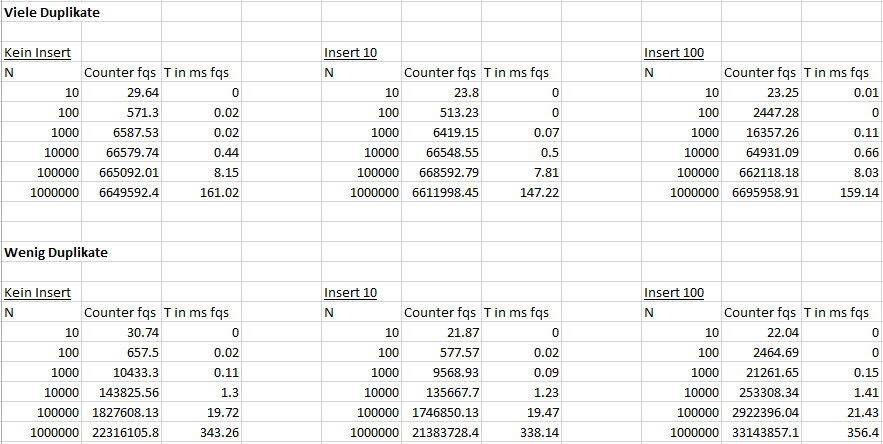
\includegraphics[width=\linewidth]{insertiontable.png}
\caption{Durchschnittswerte unterschiedlicher Insertionsorts von 100 Durchführungen bei vielen und wenigen Duplikaten}
\label{figure:table}
\end{figure}
\end{document}